\chapter{Déploiement du Système d'information}
%\markboth{Chapitre 3 }{Déploiement du Système d'information} %pour afficher l'entete
 %\addcontentsline{toc}{chapter}{Chapitre 3 : Déploiement du Système d'information}


\section{Introduction}


Le déploiement du système d'information est une étape cruciale pour toute entreprise moderne. Afin de répondre aux besoins spécifiques de Zeta Engineering, nous avons identifié les éléments essentiels à intégrer dans notre système d'information, tels que les protocoles de communication et les serveurs. 


Dans ce chapitre, nous détaillons les différentes étapes du déploiement de ce système d'information, en commençant par l'installation et la configuration des serveurs nécessaires à leur fonctionnement. Nous expliquons également les choix techniques que nous avons effectués pour répondre aux exigences de l'entreprise et assurer une infrastructure robuste et sécurisée \cite{opg}.


\section{Les besoins de notre système d'information}



Dans cette section, nous montrons les besoins essentielles de notre entreprise.



\begin{table}[H]
\begin{center}
\begin{tabular}{|c{3cm}|l{10cm}|}
\hline
\textbf{Besoin} & \begin{center} \textbf{Description} \end{center} \\
\hline
OS Serveur & Système d'exploitation spécialement conçu pour les serveurs, offrant des fonctionnalités de stabilité, de performance et de compatibilité avec divers logiciels et technologies. \\
\hline
Virtualisation & Permettre l'exécution de systèmes virtuels sur différents systèmes d'exploitation en simulant du matériel standardisé. \\
\hline
Protocole de communication & Ensemble de règles et de conventions permettant à différents composants du réseau de communiquer entre eux de manière cohérente. \\
\hline
ERP/CRM & Plateforme intégrée de gestion d'entreprise qui offre des fonctionnalités pour la gestion des ressources, des ventes, des finances, des ressources humaines et bien plus encore. \\
\hline
Système de téléphonie IP & Gérer les appels téléphoniques, y compris la gestion des lignes et d'autres fonctionnalités avancées. Il prend en charge différents protocoles de communication, tels que SIP et RTP, permettant ainsi la mise en place de communications vocales à travers le réseau IP. \\
\hline
Gestion de parc et d'inventaires & Suivre et gérer les actifs matériels et logiciels d'une organisation, y compris les utilisateurs, les ordinateurs, les périphériques et les licences logicielles. \\
\hline
Gestion des identités et contrôle d'accès & Gérer les utilisateurs, les ordinateurs et les groupes au sein d'un réseau. Fournir des fonctionnalités d'authentification, de contrôle d'accès et de gestion des politiques de sécurité. \\
\hline
\end{tabular}
\caption{Les éléments composants le système d'information}
\label{1}
\end{center}
\end{table}


\section{Les solutions choisies}

Dans cette section, nous présentons les solutions essentielles que nous avons choisies pour intégrer le système d’information de notre entreprise.

\subsection{OS Serveur}

Nous choisissons Ubuntu Server 22.04 comme système d'exploitation pour nos serveurs en raison de ses performances exceptionnelles, de sa stabilité prouvée et de sa compatibilité avec de nombreux logiciels et technologies. Ubuntu Server est une distribution Linux conçue spécialement pour les serveurs, ce qui en fait un choix optimal pour notre environnement.

La version 22.04 d'Ubuntu Server est la dernière itération de cette distribution basée sur le noyau Linux. Elle offre plusieurs améliorations et fonctionnalités, notamment :

\begin{itemize}


\item Des performances accrues : Ubuntu Server 22.04 est optimisé pour offrir des performances élevées, permettant de gérer efficacement même les charges de travail les plus exigeantes.

\item Une sécurité renforcée : Cette distribution intègre des fonctionnalités de sécurité avancées, telles que la prise en charge du chiffrement des données, des mises à jour automatiques et la gestion des certificats pour garantir la confidentialité et l'intégrité des données.

\item Support à long terme : Ubuntu Server 22.04 bénéficie d'un support à long terme (LTS) de cinq ans, ce qui signifie que des mises à jour de sécurité et des correctifs seront disponibles sur une période prolongée, assurant ainsi la stabilité et la fiabilité du système.

\item Écosystème riche : Ubuntu Server est soutenu par une communauté active d'utilisateurs et de développeurs, offrant un soutien abondant, une documentation complète et une large gamme de logiciels et d'outils pour répondre aux besoins spécifiques de nos serveurs.


\end{itemize}

\subsection{Virtualisation}

Nous choisissons KVM (Kernel-based Virtual Machine) pour la virtualisation de nos serveurs en raison de ses avantages significatifs. KVM est une technologie de virtualisation open source qui permet l'exécution de plusieurs machines virtuelles sur un seul serveur physique. Les avantages de cette solution sont les suivants :

\begin{itemize}

\item Efficacité et performances : KVM est intégré au noyau Linux, ce qui lui confère une grande efficacité et des performances élevées. Il tire pleinement parti des ressources matérielles du serveur, assurant ainsi une expérience de virtualisation fluide.

\item Isolation et sécurité : KVM garantit une isolation totale entre les machines virtuelles, assurant la sécurité des données et des applications. Chaque machine virtuelle fonctionne de manière indépendante, réduisant ainsi les risques de failles de sécurité.

\item Compatibilité : KVM est compatible avec divers systèmes d'exploitation invités, ce qui permet d'exécuter différents environnements logiciels au sein de machines virtuelles distinctes.

\item Évolutivité : La virtualisation avec KVM est hautement évolutive. Nous pouvons ajouter ou supprimer des machines virtuelles selon les besoins de votre entreprise sans perturber les opérations en cours.

\end{itemize}




\subsection{Protocole de communication}

Pour gérer les adresses IP de notre réseau, nous optons pour ISC DHCP (Internet Systems Consortium - Dynamic Host Configuration Protocol). ISC DHCP est un protocole de communication qui joue un rôle essentiel dans l'attribution automatique des adresses IP aux dispositifs connectés à notre réseau. Voici les raisons de ce choix :

\begin{itemize}

\item Fiabilité : ISC DHCP est largement reconnu pour sa fiabilité. Il assure une distribution efficace des adresses IP tout en minimisant les conflits d'adresses et les interruptions de réseau.

\item Facilité de gestion : La configuration et la gestion d'ISC DHCP sont conviviales, ce qui simplifie la maintenance de notre réseau. Nous pouvons aisément définir des plages d'adresses, des options de configuration personnalisées et surveiller l'état du service DHCP.

\item Prise en charge des protocoles : ISC DHCP prend en charge plusieurs protocoles de communication, notamment IPv4 et IPv6. Cela garantit la compatibilité avec divers dispositifs et systèmes d'exploitation.

\item Évolutivité : Notre choix d'ISC DHCP est évolutif, ce qui signifie que nous pouvons facilement adapter notre réseau aux besoins croissants de notre entreprise en ajoutant de nouveaux dispositifs sans soucis de gestion des adresses IP.

\end{itemize}

Ce protocole de communication joue un rôle crucial dans l'attribution et la gestion des adresses IP au sein de notre réseau, assurant ainsi une connectivité fiable pour tous nos dispositifs.

\subsection{ERP/CRM}

Pour les plates-formes ERP/CRM, nous sélectionnons Odoo. Odoo est une solution intégrée de gestion d'entreprise qui offre une gamme complète de fonctionnalités pour la gestion des ressources, des ventes, des finances, des ressources humaines et bien plus encore. Notre choix d'Odoo repose sur plusieurs avantages clés :

\begin{itemize}

\item Intégration complète : Odoo propose une intégration complète de toutes les fonctions essentielles de l'entreprise. Cela signifie que nous pouvons gérer divers aspects de notre entreprise, tels que la comptabilité, les ventes, les stocks et la gestion des projets, à partir d'une seule plate-forme centralisée.

\item Personnalisation : Odoo est hautement personnalisable, ce qui nous permet d'adapter la plate-forme à nos besoins spécifiques. Nous pouvons personnaliser les flux de travail, les rapports et les tableaux de bord pour répondre à nos exigences métier uniques.

\item Facilité d'utilisation : Odoo est réputé pour sa convivialité. Notre équipe pourra rapidement prendre en main la plate-forme, ce qui réduira la courbe d'apprentissage et favorisera une utilisation optimale.

\item Communauté active : Odoo bénéficie d'une communauté mondiale active d'utilisateurs et de développeurs. Cela signifie que nous avons accès à une vaste base de connaissances, à des modules complémentaires personnalisés et à un support communautaire en cas de besoin.

\end{itemize}

Avec Odoo comme plate-forme ERP/CRM, nous disposons d'un outil puissant pour optimiser nos opérations commerciales, améliorer notre gestion des clients et devenir plus efficaces dans l'ensemble de notre entreprise.



\subsection{Système de téléphonie IP}

Pour notre système de téléphonie IP, notre choix se porte sur Asterisk, une solution de gestion des appels téléphoniques au sein de notre entreprise. Cette décision repose sur plusieurs avantages clés :

\begin{itemize}


\item Flexibilité : Asterisk est reconnu pour sa grande souplesse. Il prend en charge divers protocoles de communication, tels que SIP et RTP, nous permettant ainsi d'établir des communications vocales via notre réseau IP.

\item Fonctionnalités avancées : Asterisk propose une vaste gamme de fonctionnalités avancées pour la gestion des appels téléphoniques. Cela englobe la gestion des lignes, la messagerie vocale, les conférences téléphoniques, et bien plus encore.

\item Personnalisation : Asterisk est hautement personnalisable. Nous avons la possibilité d'ajuster le système en fonction de nos besoins spécifiques, créant ainsi une solution de téléphonie sur mesure pour notre entreprise.

\item Économies de coûts : L'utilisation d'Asterisk se traduit par des économies significatives sur nos frais de communication. La téléphonie IP est généralement plus rentable que les systèmes de téléphonie traditionnels.


\end{itemize}

En choisissant Asterisk comme solution de téléphonie IP, nous sommes en mesure de mettre en place une infrastructure de communication vocale moderne et adaptable pour répondre aux besoins de notre entreprise.




\subsection{Gestion de parc et d'inventaires}

Pour la gestion de parc et d'inventaires, nous choisissons GLPI avec l'intégration de FusionInventory. Cette solution nous permet de suivre et de gérer efficacement les actifs matériels et logiciels au sein de notre organisation. Notre choix de GLPI et FusionInventory repose sur plusieurs avantages clés :

\begin{itemize}

\item Suivi complet des actifs : GLPI nous offre la possibilité de suivre de manière exhaustive tous les actifs de notre parc, y compris les ordinateurs, les périphériques, les logiciels, et bien plus encore. Cela garantit une gestion précise de nos ressources.

\item Gestion des utilisateurs : GLPI nous permet de gérer les utilisateurs au sein de notre réseau de manière efficace. Nous pouvons attribuer des actifs aux utilisateurs et suivre leur utilisation de manière transparente.

\item Automatisation des tâches : FusionInventory, intégré à GLPI, automatise de nombreuses tâches de gestion, telles que l'inventaire des actifs et la gestion des mises à jour. Cela nous fait gagner du temps et améliore la précision des données.

\item Personnalisation : GLPI est hautement personnalisable pour répondre à nos besoins spécifiques. Nous pouvons adapter les champs et les processus pour une gestion des actifs sur mesure.

\end{itemize}

Avec GLPI et FusionInventory, nous avons la capacité de gérer de manière efficace l'ensemble de nos actifs, de suivre les changements, et d'optimiser l'utilisation de nos ressources.




\subsection{Gestion des identités et contrôle d'accès}

Pour la gestion des identités et le contrôle d'accès, nous avons choisi OpenLDAP en raison de son caractère open source, de sa flexibilité et de sa robustesse. OpenLDAP est une solution de répertoire qui nous permet de gérer les identités des utilisateurs, les groupes et les autorisations d'accès au sein de notre infrastructure informatique. Voici plusieurs raisons convaincantes qui motivent notre choix d'OpenLDAP :

\begin{itemize}


\item Gratuit et Open Source : OpenLDAP est une solution open source, ce qui signifie qu'elle est disponible gratuitement. Cela correspond parfaitement à notre souci de maîtriser les coûts tout en bénéficiant de fonctionnalités avancées.

\item Personnalisable : OpenLDAP offre une grande souplesse en matière de personnalisation, nous permettant de configurer des schémas et des attributs spécifiques en fonction de nos besoins. Nous pouvons ainsi adapter la structure du répertoire à notre organisation.

\item Interopérabilité : OpenLDAP prend en charge les protocoles LDAP standards, facilitant ainsi son intégration avec d'autres applications et services. Nous pouvons l'utiliser pour centraliser l'authentification et l'autorisation sur diverses plateformes.

\item Fonctionnalités de sécurité : OpenLDAP propose des fonctionnalités de sécurité robustes, notamment une authentification renforcée, le chiffrement des données et la gestion des politiques d'accès. Cela garantit la protection de nos données sensibles.

\item Engagement de la communauté : OpenLDAP reçoit le soutien d'une communauté dynamique d'utilisateurs et de développeurs, ce qui garantit un appui constant, un accès à des ressources utiles et des mises à jour fréquentes.


\end{itemize}


Avec OpenLDAP, nous mettons en place un système solide et sécurisé de gestion des identités, répondant à nos besoins en matière de contrôle d'accès et d'authentification au sein de notre infrastructure informatique.



\section{Déploiement des solutions choisies}

Nos solutions choisies se répartissent en trois couches distinctes, comme illustré dans la figure \ref{fig:diagramme-SI}. La couche inférieure représente la couche physique, où nous installons le système d'exploitation serveur. Au-dessus, nous avons la couche de virtualisation, où nous créons des environnements virtuels pour nos applications. Enfin, la couche supérieure est la couche applicative, où nous déployons nos machines virtuelles et exécutons nos applications.


\begin{figure}[H]
\centering
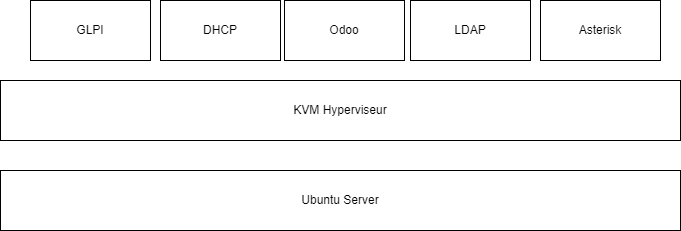
\includegraphics[width=16cm]{Images/diagsi.png}
\caption{Diagramme du système d'information}
\label{fig:diagramme-SI}
\end{figure}






\subsection{La couche physique}

La configuration de la couche physique de notre infrastructure s'est déroulée en suivant scrupuleusement le guide d'installation d'Ubuntu Server 22.04 \cite{linuxgenie_ubuntu2204}. 

\begin{figure}[H]
  \centering
  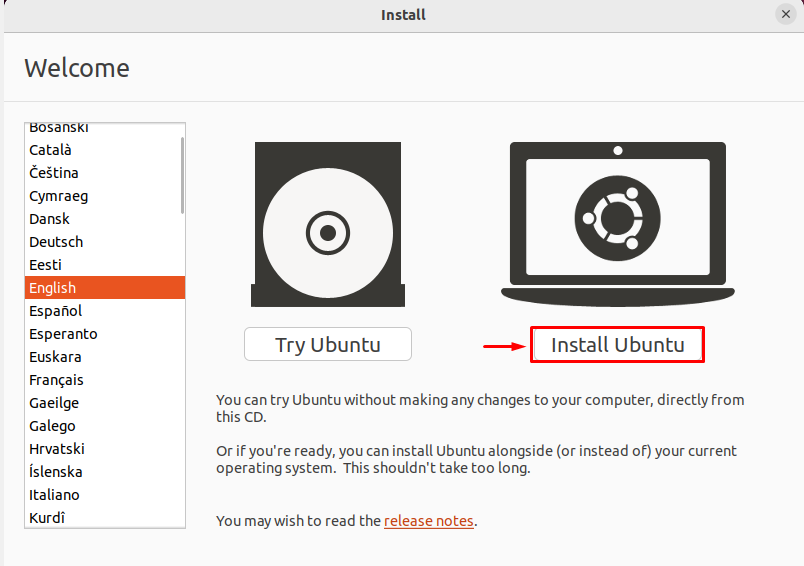
\includegraphics[width=15cm]{Images/ubuntu-install.png}
  \caption{Installation de Ubuntu Server 22.04}
  \label{fig:ubuntu-install}
\end{figure}

La figure \ref{fig:ubuntu-install} illustre notre procédure d'installation d'Ubuntu Server.

\begin{figure}[H]
  \centering
  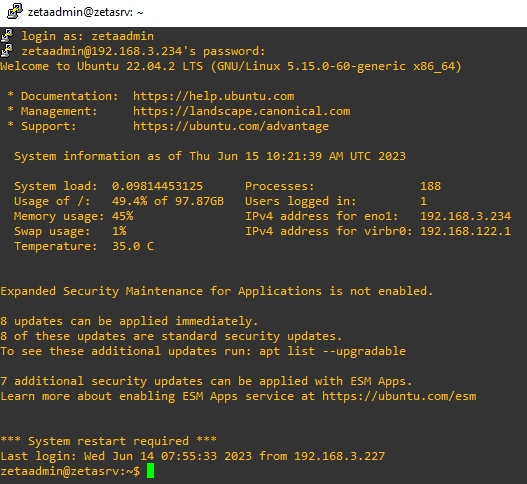
\includegraphics[width=15cm]{Images/zetaserver.png}
  \caption{Interface Putty pour la connexion à Ubuntu Server 22.04}
  \label{fig:putty-interface}
\end{figure}

Dans la figure \ref{fig:putty-interface}, nous exposons en détail l'interface de Putty, l'outil que nous employons pour effectuer la connexion à notre serveur Ubuntu 22.04. Cette interface est l'interface de contrôle permettant la gestion à distance de notre serveur.

\begin{figure}[H]
  \centering
  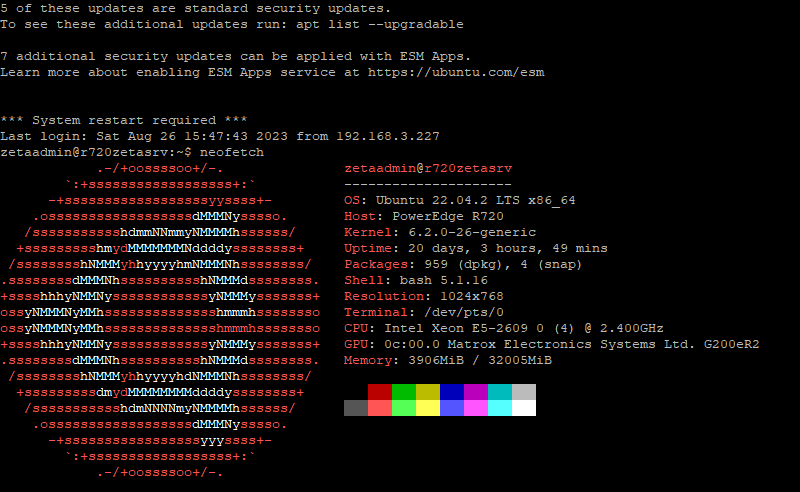
\includegraphics[width=15cm]{Images/neofetchzetasrv1.png}
  \caption{Résultat de la commande "neofetch" sur Ubuntu Server 22.04}
  \label{fig:neofetch-result}
\end{figure}

La figure \ref{fig:neofetch-result} affiche le résultat détaillé de l'exécution de la commande "neofetch" sur notre serveur Ubuntu 22.04. Cette commande nous a permis d'obtenir des informations système essentielles pour assurer le bon fonctionnement de notre infrastructure.


\subsection{La couche virtualisation}

Avant d'installer KVM, nous effectuons des vérifications pour garantir la compatibilité matérielle. 

Tout d'abord, nous exécutons la commande \textbf{egrep -c '(vmx|svm)' /proc/cpuinfo} pour vérifier la présence des instructions de virtualisation matérielles (VT-x pour Intel ou AMD-V pour AMD) sur le processeur. Un résultat supérieur à zéro indique que le processeur prend en charge la virtualisation matérielle.

Ensuite, nous utilisons la commande \textbf{kvm-ok} pour vérifier si les modules de virtualisation étaient correctement chargés dans le système et si la virtualisation était prise en charge.

Une fois ces vérifications réussies, nous procédons à l'installation des packages nécessaires en exécutant la commande suivante :


\textbf{"sudo apt install -y qemu-kvm virt-manager libvirt-daemon-system virtinst libvirt-clients bridge-utils"}

\begin{itemize}
\item  qemu-kvm est l'hyperviseur qui permet l'exécution de machines virtuelles, fournissant un environnement pour les systèmes d'exploitation invités.
\item virt-manager est une interface graphique conviviale qui facilite la gestion des machines virtuelles, offrant des fonctionnalités de création, de configuration et de surveillance.
\item libvirt-daemon-system inclut les démons de libvirt, essentiels pour la gestion des connexions et des machines virtuelles.
\item virtinst est un outil en ligne de commande qui permet la création et la gestion des machines virtuelles de manière efficace.
\item libvirt-clients englobe des outils en ligne de commande qui permettent d'interagir avec le démon libvirt pour le contrôle des VM.
\item bridge-utils est un package essentiel pour gérer les ponts réseau, permettant ainsi la configuration de la connectivité réseau des machines virtuelles.
\end{itemize}









Ci-dessous, nous pouvons voir que les figures \ref{fig:kvm-installation} et \ref{fig:libvirtd-status} illustrant les étapes d'installation de KVM et la vérification de l'état du service libvirtd  .

\begin{figure}[H]
 \centering
    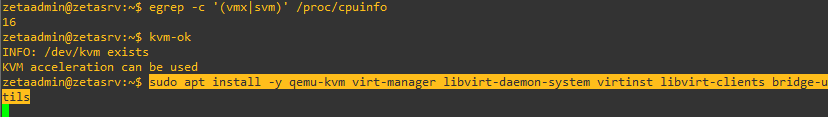
\includegraphics[width=15cm]{Images/installkvm1.png}
    \caption{Installation des packages KVM}
    \label{fig:kvm-installation}
\end{figure}

\begin{figure}[H]
 \centering
    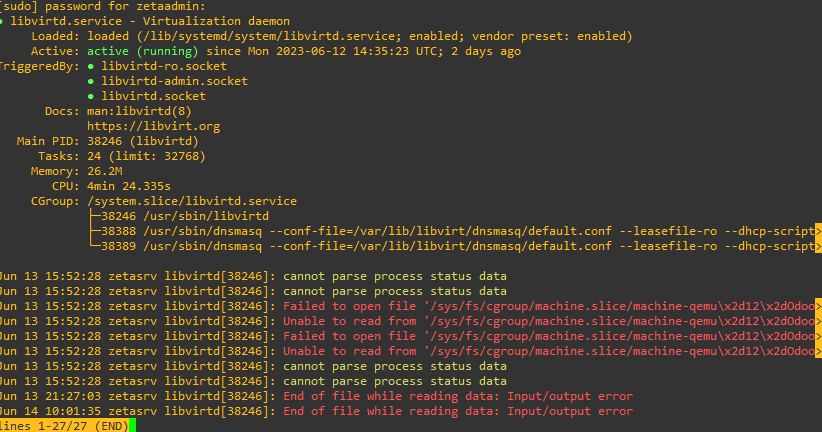
\includegraphics[width=15cm]{Images/installkvm2.png}
    \caption{Vérification de l'état du service libvirtd}
    \label{fig:libvirtd-status}
\end{figure}

Enfin, grâce à l'utilisation de Xming et de PuTTY, nous pouvons accéder au gestionnaire graphique Virt-Manager à distance depuis notre utilisateur Windows, comme illustré dans la figure \ref{fig:virt-manager-access}. Cela nous permet de configurer nos machines virtuelles de manière conviviale.

\begin{figure}[H]
 \centering
    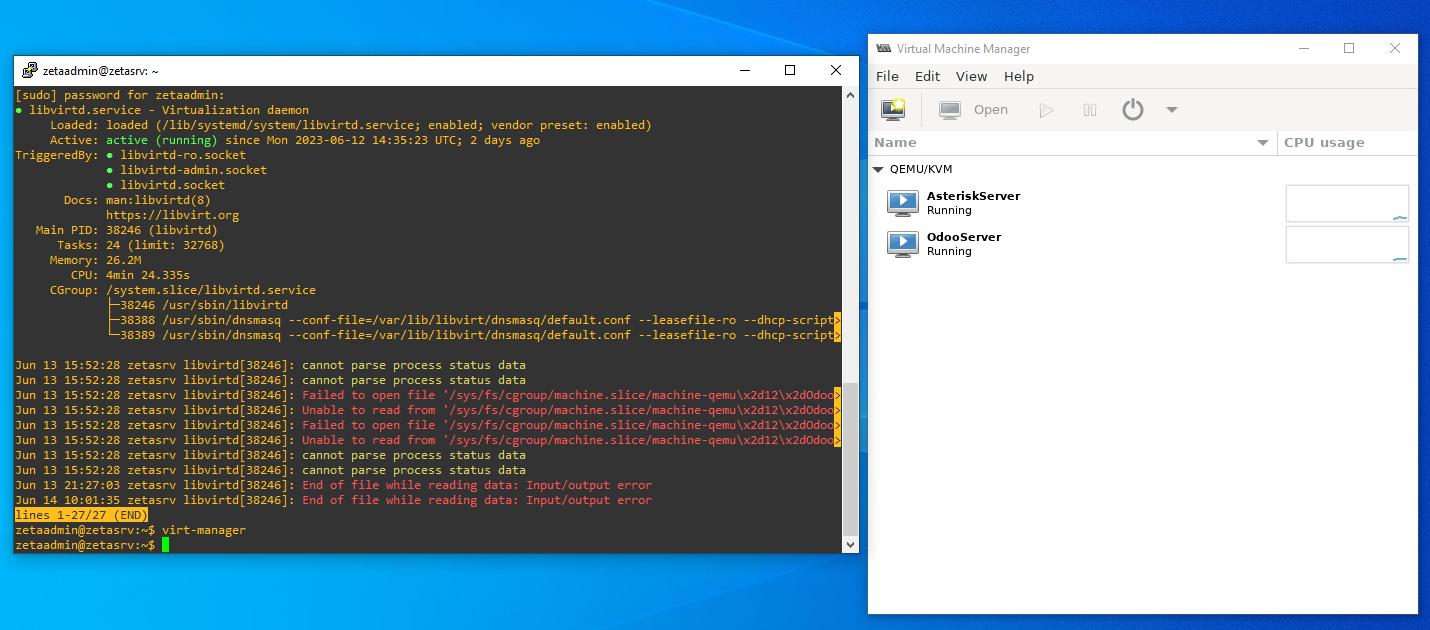
\includegraphics[width=15cm]{Images/resultvirtmanager.png}
    \caption{Accès à Virt-Manager via Xming et PuTTY}
    \label{fig:virt-manager-access}
\end{figure}

\subsection{La couche applicative}

\subsubsection{a. DHCP}

Pour mettre en place et configurer un serveur DHCP sur une machine virtuelle Linux, nous avons suivi les étapes suivantes \cite{linuxhint_dhcp_server}.

Tout d'abord, nous effectuons une mise à jour du système Linux en exécutant la commande \textbf{"apt-get update"} comme illustré dans la figure \ref{fig:update-linux}.

\begin{figure}[H]
    \centering
    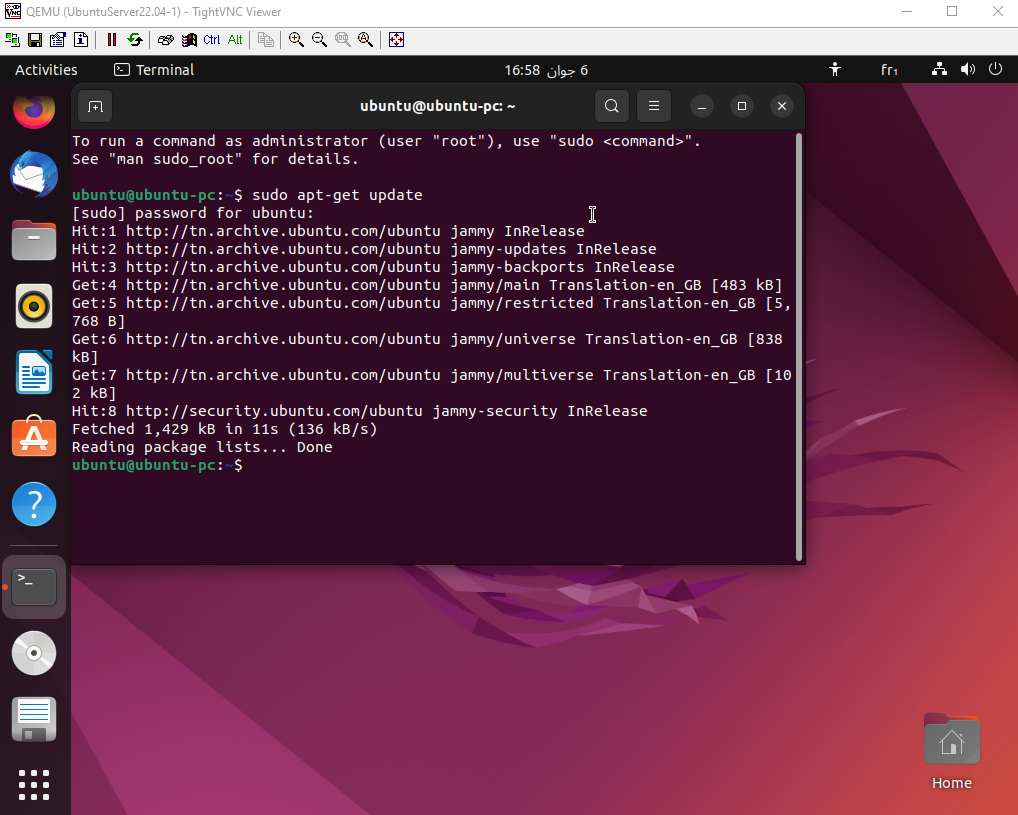
\includegraphics[width=0.8\textwidth]{Images/dhcp1.png}
    \caption{Mise à jour du système Linux}
    \label{fig:update-linux}
\end{figure}

Ensuite, nous redémarrons le service isc-dhcp pour appliquer les modifications, comme le montre la figure \ref{fig:restart-isc-dhcp}.

\begin{figure}[H]
    \centering
    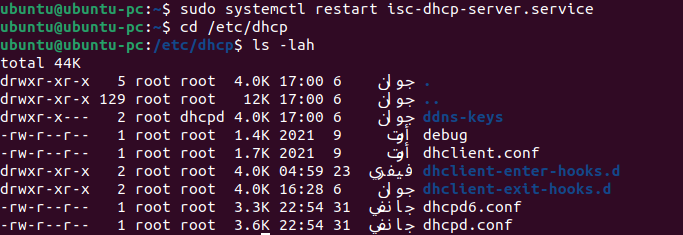
\includegraphics[width=0.8\textwidth]{Images/dhcp2.png}
    \caption{Redémarrage du service isc-dhcp}
    \label{fig:restart-isc-dhcp}
\end{figure}

Nous procédons ensuite à la configuration du fichier dhcpd.conf à l'aide de l'éditeur de texte gedit, comme indiqué dans la figure \ref{fig:dhcpd-conf-configuration}.

\begin{figure}[H]
    \centering
    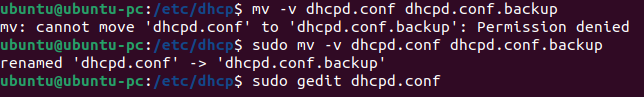
\includegraphics[width=0.8\textwidth]{Images/dhcp3.png}
    \caption{Configuration du fichier \texttt{dhcpd.conf}}
    \label{fig:dhcpd-conf-configuration}
\end{figure}

La figure  \ref{fig:dhcpd-conf-example} illustre un exemple de fichier de configuration \texttt{dhcpd.conf}.

\begin{figure}[H]
    \centering
    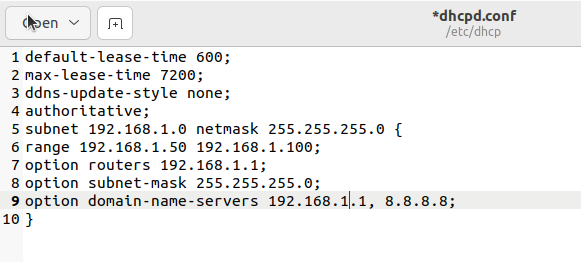
\includegraphics[width=0.8\textwidth]{Images/dhcp4.png}
    \caption{Exemple de fichier de configuration \texttt{dhcpd.conf}}
    \label{fig:dhcpd-conf-example}
\end{figure}

Enfin, nous vérifions que le serveur DHCP ISC était en cours d'exécution en utilisant la commande \textbf{"systemctl status isc-dhcp-server.service"}, comme montré dans la figure \ref{fig:isc-dhcp-service-status}.

\begin{figure}[H]
    \centering
    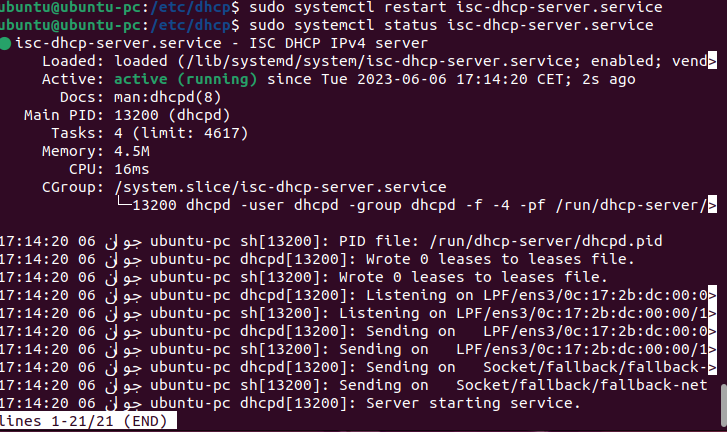
\includegraphics[width=0.8\textwidth]{Images/dhcp5.png}
    \caption{État du service ISC DHCP}
    \label{fig:isc-dhcp-service-status}
\end{figure}

Ainsi, nous réussissons  à mettre en place et configurer un serveur DHCP sur notre machine virtuelle Linux. Cela nous permettra de fournir automatiquement des adresses IP et d'autres informations de configuration réseau aux clients DHCP de notre réseau.

\subsubsection{b. VoIP/Téléphonie}

Après avoir suivi les étapes d'installation d'Asterisk \cite{asterisk-install-vegastack}, comme illustré dans la figure \ref{fig:asterisk-server1}, notre système Asterisk fonctionne correctement.

\begin{figure}[H]
    \centering
    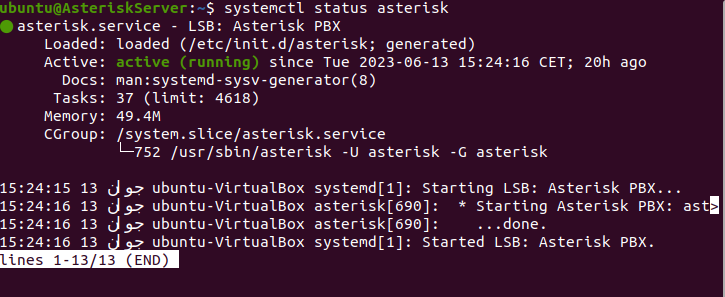
\includegraphics[width=0.8\textwidth]{Images/AsteriskServer1.png}
    \caption{Installation d'Asterisk sur Ubuntu}
    \label{fig:asterisk-server1}
\end{figure}


\subsubsection{c. ERP/CRM}

L'installation d'Odoo \cite{odoo16-ubuntu-install} sur notre machine virtuelle Ubuntu.


Nous poursuivons avec la configuration et la vérification d'Odoo en utilisant PostgreSQL. La figure \ref{fig:psql-version} affiche le résultat de la commande "systemctl status odoo15" et "psql --version," confirmant ainsi la compatibilité d'Odoo avec PostgreSQL.

\begin{figure}[H]
\centering
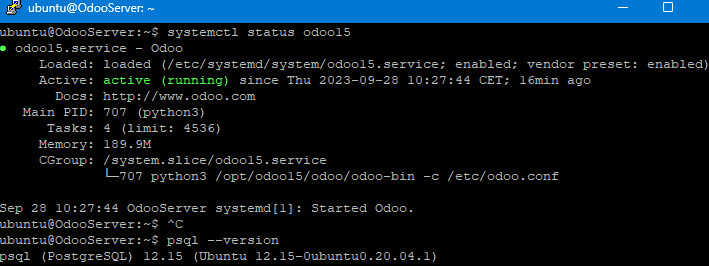
\includegraphics[width=15cm]{Images/post104722.png}
\caption{Configuration d'Odoo et version PostgreSQL}
\label{fig:psql-version}
\end{figure}

De plus, pour assurer l'intégration réussie avec PostgreSQL, nous présentons la figure \ref{fig:Dashboard-Odoo-DB} qui montre la base de données PostgreSQL dans le tableau de bord d'Odoo.

\begin{figure}[H]
\centering
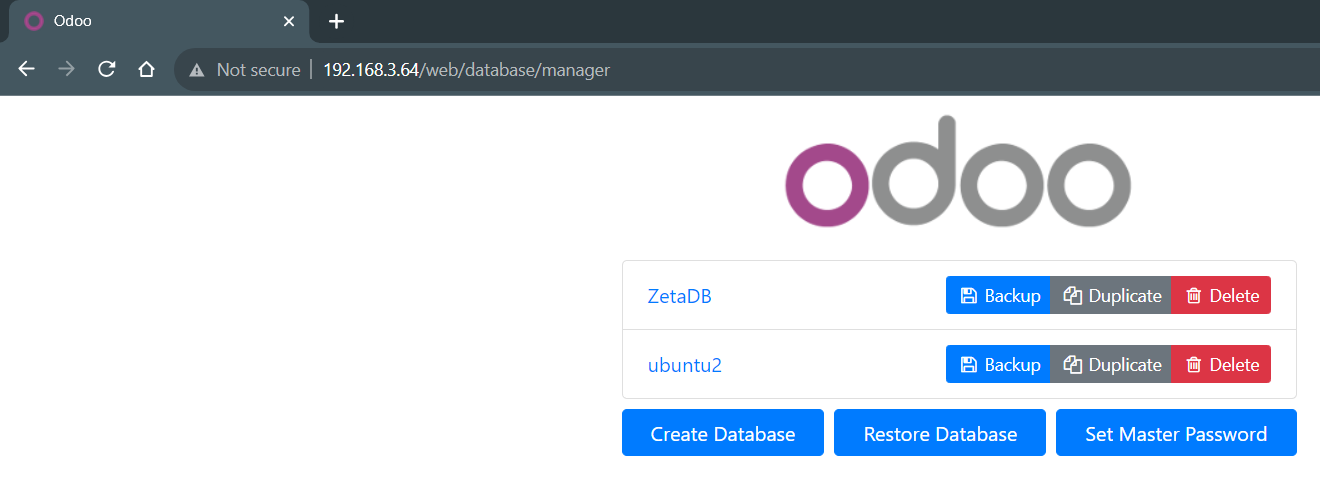
\includegraphics[width=15cm]{Images/104614.png}
\caption{Base de données PostgreSQL dans le tableau de bord Odoo}
\label{fig:Dashboard-Odoo-DB}
\end{figure}

Enfin, pour confirmer le bon fonctionnement d'Odoo et sa compatibilité avec PostgreSQL, nous affichons le tableau de bord d'Odoo avec les modules CRM installés dans la figure \ref{fig:odoo-dashboard}.

\begin{figure}[H]
\centering
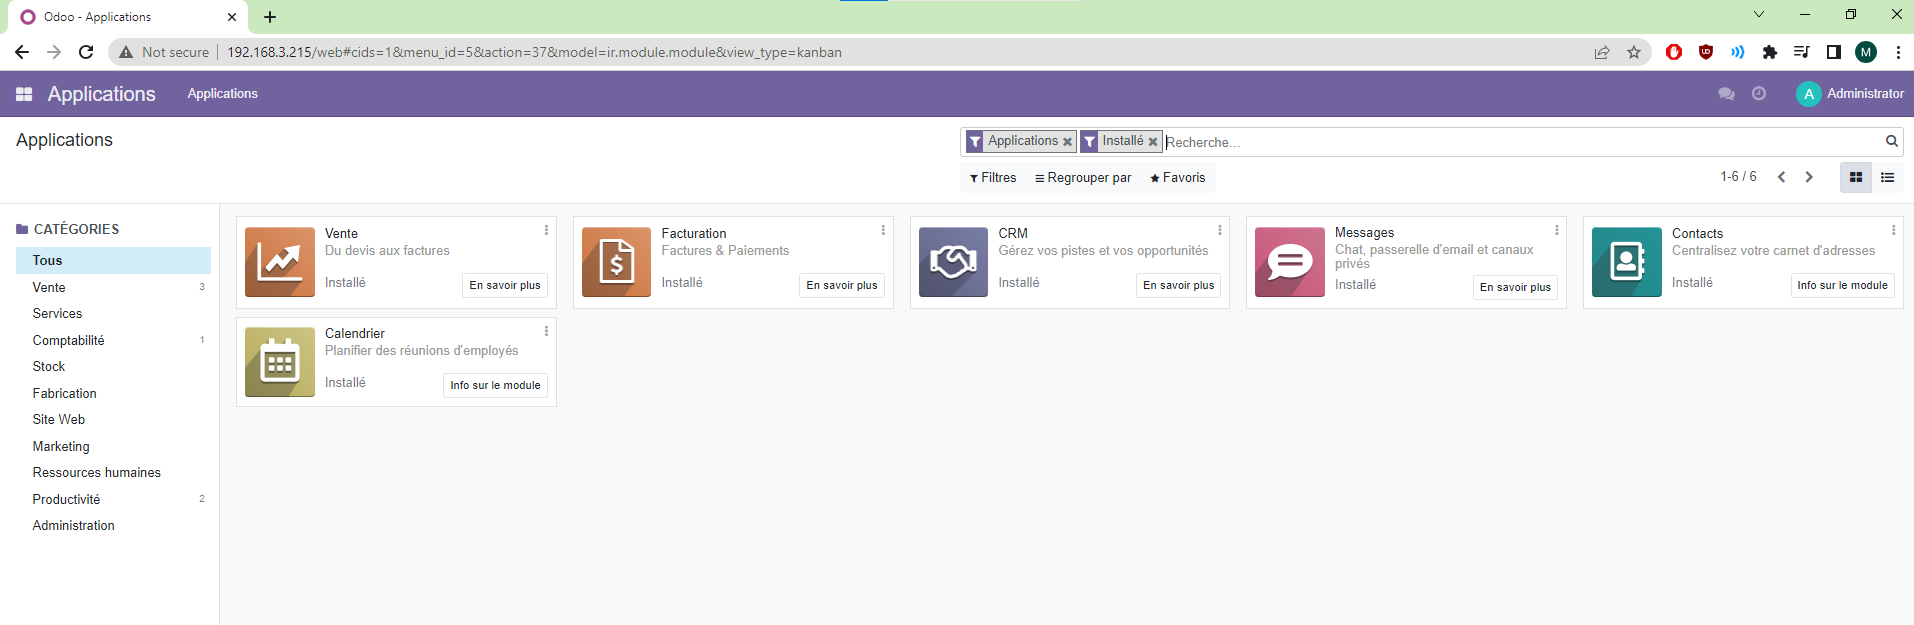
\includegraphics[width=15cm]{Images/OdooServer2.png}
\caption{Tableau de bord d'Odoo avec les modules CRM installés}
\label{fig:odoo-dashboard}
\end{figure}



\subsubsection{d. GLPI}

L'installation de GLPI \cite{glpi-install-tecmint} est suivie d'un aperçu du tableau de bord de GLPI, où toutes les informations sur les équipements peuvent être consultées et gérées efficacement, comme montré dans la figure \ref{fig:glpi-dashboard}.


\begin{figure}[H]
\centering
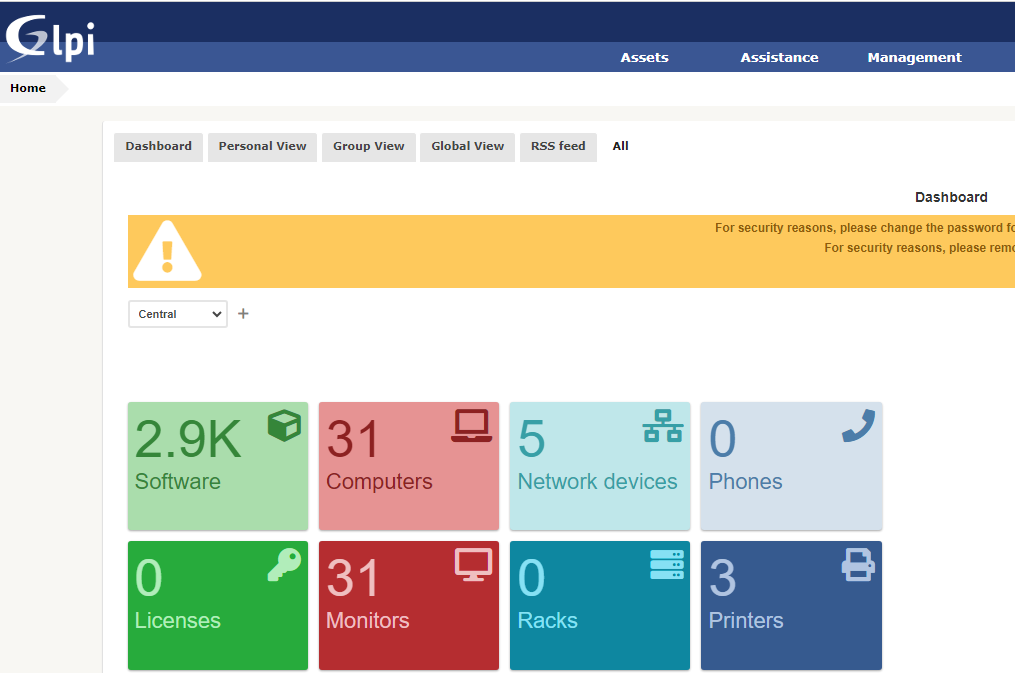
\includegraphics[width=15cm]{Images/GLPI.png}
\caption{Tableau de bord de GLPI}
\label{fig:glpi-dashboard}
\end{figure}

Pour intégrer harmonieusement GLPI dans notre infrastructure, nous ajoutons une base de données MariaDB. MariaDB est un choix judicieux en raison de sa compatibilité et de ses performances élevées. La figure \ref{fig:Putty-MARIADB-SHOWTABLES} témoigne du bon fonctionnement de notre système avec l'affichage de "SHOW TABLES;". Cette étape garantit que GLPI est prêt à être utilisé dans notre environnement pour gérer les informations sur les équipements de manière efficace.


\begin{figure}[H]
\centering
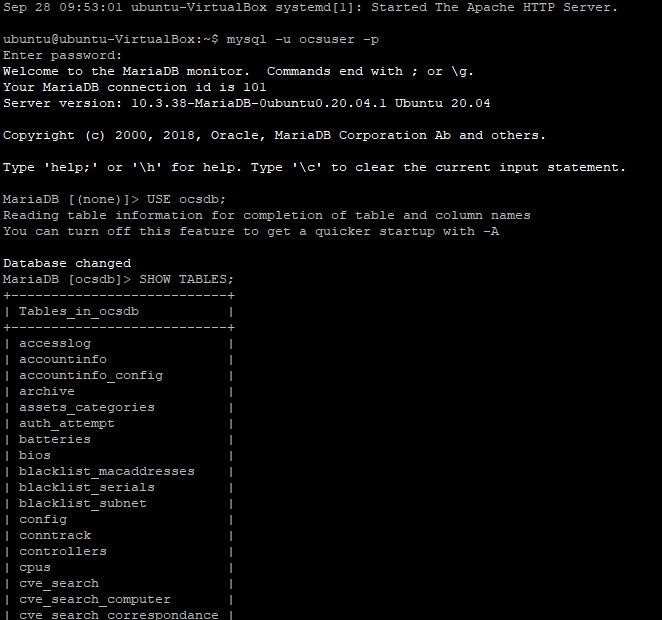
\includegraphics[width=15cm]{Images/20230928102651.png}
\caption{Affichage des tables dans MariaDB}
\label{fig:Putty-MARIADB-SHOWTABLES}
\end{figure}


\subsubsection{e. OpenLDAP}

Après avoir suivi les étapes pour installer OpenLDAP \cite{patil2020openldap}, nous présentons le tableau de bord de phpLDAPAdmin, une interface graphique pour la gestion de l'annuaire LDAP \ref{fig:ldap-dashboard}.

\begin{figure}[H]
\centering
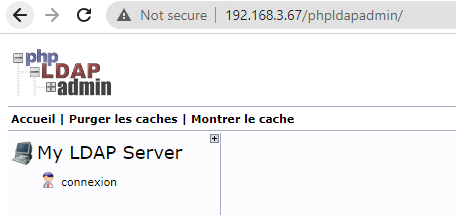
\includegraphics[width=15cm]{Images/ldapdashboard.png}
\caption{Tableau de bord de phpLDAPAdmin}
\label{fig:ldap-dashboard}
\end{figure}

\subsubsection{f. Les machines virtuelles de nos applications}


\begin{figure}[H]
\centering
\includegraphics[width=15cm]{Images/virsh-listall.png}
\caption{Liste des machines virtuelles déployées}
\label{fig:vm-list}
\end{figure}

La figure \ref{fig:vm-list} présente la liste complète de nos VMs actuellement déployées, chacune d'entre elles étant dédiée à l'une de nos applications. Ce déploiement nous permet de garantir l'isolation des ressources et de maintenir la disponibilité de nos applications de manière efficace.



\section{Conclusion}

Le système d'information de Zeta Engineering est déployé de manière structurée, en utilisant des solutions adaptées : Ubuntu Server 22.04 comme OS serveur, KVM pour la virtualisation, DHCP ISC DHCP pour la gestion des IP, Odoo pour la gestion d'entreprise, Asterisk pour les appels, GLPI et FusionInventory pour l'inventaire, et OpenLDAP pour l'identité.

L'installation et la configuration suivent des étapes précises. Ubuntu Server est choisi pour sa performance et sa compatibilité. KVM héberge les VM, DHCP ISC DHCP gère les IP, Odoo centralise la gestion, et Asterisk prend en charge les appels.

Ce déploiement crée une base solide et sécurisée. L'équipe informatique peut maintenant optimiser le système pour les besoins en constante évolution de l'entreprise.

En conclusion, ce déploiement garantit le bon fonctionnement efficace et fiable de Zeta Engineering. Nous passerons maintenant au dernier chapitre, où nous aborderons l'intégration des objets connectés.




